\documentclass[graybox]{svmult}

% choose options for [] as required from the list
% in the Reference Guide

\usepackage{mathptmx}       % selects Times Roman as basic font
\usepackage{helvet}         % selects Helvetica as sans-serif font
\usepackage{courier}        % selects Courier as typewriter font
\usepackage{type1cm}        % activate if the above 3 fonts are
                             % not available on your system
%
\usepackage{makeidx}         % allows index generation
\usepackage{graphicx}        % standard LaTeX graphics tool
                             % when including figure files
\usepackage{multicol}        % used for the two-column index
\usepackage[bottom]{footmisc}% places footnotes at page bottom
\usepackage{latexsym,amsmath,amssymb,bm,booktabs,epsfig,multirow,bigstrut,graphicx,url,natbib}
%\usepackage{nath}

% see the list of further useful packages
% in the Reference Guide

\makeindex             % used for the subject index
                       % please use the style svind.ist with
                       % your makeindex program
                       
\input FJHDef.tex
%\renewcommand{\bvec}[1]{\textbf{\itshape #1}}
%\renewcommand{\bvec}[1]{\boldsymbol{#1}}
\newcommand{\cube}{[0,1)^d}
\newcommand{\tcube}{\widetilde{[0,1)}^d}
\newcommand{\hv}{\hat{v}}
\newcommand{\fudge}{\mathfrak{C}}
\DeclareMathOperator{\MSE}{MSE}
\DeclareMathOperator{\RMSE}{RMSE}
\DeclareMathOperator{\rnd}{rnd}
\DeclareMathOperator{\abso}{abs}
\DeclareMathOperator{\rel}{rel}
\DeclareMathOperator{\nor}{nor}
\DeclareMathOperator{\err}{err}
%\DeclareMathOperator{\prob}{prob}
\DeclareMathOperator{\third}{third}
\DeclareMathOperator{\qse}{qse}
\DeclareMathOperator{\card}{card}
%\DeclareMathOperator{\fourth}{fourth}
%\newtheorem{theorem}{Theorem}
\newtheorem{prop}[theorem]{Proposition}
\DeclareMathOperator{\sMC}{sMC}
\DeclareMathOperator{\aMC}{aMC}
\begin{document}


\date{\today}
\title*{Monte Carlo Algorithms Where the Integrand Size Is Unknown
\thanks{The first author were partially supported by the National
Science Foundation under DMS-1115392}}
\titlerunning{Adaptive Monte Carlo}
\author{Fred J. Hickernell\inst{1} \and
Lan Jiang\inst{1} \and Yuewei Liu\inst{2} \and Art Owen \inst{3}}
\institute{Department of Applied Mathematics,
Illinois Institute of Technology, Chicago, IL, USA,
\texttt{hickernell@iit.edu,ljiang14@hawk.iit.edu???other emails}
\and
School of Mathematics and Statistics, Lanzhou University, Lanzhou City, Gansu, China 730000, \texttt{???}
\and 
}
%
% Use the package "url.sty" to avoid
% problems with special characters
% used in your e-mail or web address
%
\maketitle

\abstract{We attempt a probabilistic analysis of simple Monte Carlo, achieving probabilistic error bounds when the kurtosis is controlled.  The algorithm uses a sample size that depends adaptively on the estimated variance of the integrand.  Thus, the algorithm is nonlinear (depending essentially on the function).  The advantage of what is done here over standard error analysis (complexity theory) is that the algorithm does not depend a priori on the scale of the problem (in this case the variance) to determine the number of samples.   Our intention, if what is done here is correct, is to try to extend this to the more sophisticated sampling schemes and infinite dimensional problems.}


\section{Introduction}

When one tries to utilize theoretical error bounds or complexity results for Monte Carlo integration to inform a practical algorithm, there are some real challenges.  To determine the sample size needed, one must have some information about the size of the function, specifically its standard deviation in the case of simple Monte Carlo.  Estimating this standard deviation is a step whose error is typically not analyzed.  Moreover, if one wants to guarantee that the answer obtained by the Monte Carlo algorithm satisfies a given error tolerance with a high probability, then in practice one often resorts to Central Limit Theorem, whose application also introduces an additional error that is not well understood.  

This article attempts to address these shortcomings by derving a tight theory that accounts rigorously for as much of the error in a practical algorithm as is possible.  This is done by means of some probability inequalities that involve higher moments and a variant to traditional information-based complexity theory that measures the cost of the problem in terms of the unknown size of the integrand.  

\section{Simple (I.I.D.) Monte Carlo in Practice}

\subsection{The Multivariate Integration Problem and a Practical Solution}  Suppose one wishes to compute the following integral or mean, $\mu$, of some $d$-variate function $f: \reals^d \to \reals$, i.e.,
\begin{equation*} 
\mu= \mu(f) = \int_{\reals^d} f(\vx) \rho(\vx) \, \dif \vx,
\end{equation*}
where $\rho: \reals^d \to [0,\infty)$ is a specified probability density function.  A simple Monte Carlo algorithm to estimate this integral is the sample mean of the function evaluated at independent and identically distributed random variables $\vX_1, \vX_2, \ldots$ with the marginal probability density function $\rho$:
\begin{equation} \label{samplemean}
\hmu_n = \frac 1n \sum_{i=1}^n Y_i, \qquad Y_i = f(\vX_i).
\end{equation}

A natural question is the following: \emph{How large should $n$ be to ensure with some reasonable certainty, that the absolute error of the approximation is no larger than some positive error tolerance, $\varepsilon$?}  That is, for a given a significance level or uncertainty, $\alpha$ how large should $n$ be to make 
\begin{equation} \label{abserr}
\Prob\left[\abs{\hmu_n-\mu} \le \varepsilon \right] \geq 1-\alpha.
\end{equation}
In practice, a common approach is to invoke the Central Limit Theorem, which says that
\begin{equation} \label{CLT}
\Prob\left[\abs{\hmu_n-\mu} \le \frac{z_{\alpha/2} \sigma}{\sqrt{n}} \right] \approx 1-\alpha,
\end{equation}
where $z_\alpha$ denotes the $(1-\alpha)100\%$ percentile of the standard Gaussian distribution, and $\sigma^2$ denotes the variance of the function:
\begin{equation} \label{sigmadef}
\sigma^2 := \var(Y_1) = \var(f(\vX_1)) =: \var(f) = \int_{\reals^d} \abs{f(\vx)-\mu}^2 \rho(\vx) \, \dif \vx.
\end{equation}
This variance $\sigma^2$ is typically unknown a priori, but it can be estimated in terms of the sample variance based on a  sample of size, $n_{\sigma} \in \naturals$:
\begin{equation} \label{samplevar}
\hsigma^2 = \fudge^2 \hv_{n_{\sigma}}, \quad \text{where} \quad \hv_{n_{\sigma}} = \frac 1{n_{\sigma}-1} \sum_{i=1}^{n_{\sigma}} [Y_i- \hmu_{n_{\sigma}}]^2, \quad \hmu_{n_{\sigma}} = \frac 1{n_{\sigma}} \sum_{i=1}^{n_{\sigma}} Y_i, \quad Y_i=f(\vX_i).
\end{equation}
The variance inflation factor $\fudge>1$ accounts for the fact that as an unbiased estimator, the sample variance may be larger or smaller than the true variance.  Defining 
\begin{equation} \label{CLTsample}
N_{G}(\varepsilon,\alpha) :=\left \lceil \left(\frac{z_{\alpha/2}}{\varepsilon}\right)^2 \right \rceil, 
\end{equation}
in light of the Central Limit Theorem, one then estimates the true mean by $\hmu_{n}$, based on an additional $n=N_{G}(\varepsilon/\hsigma,\alpha)$ independent samples:
\begin{equation} \label{simpleMCest}
\hmu_n = \frac 1n \sum_{i=n_{\sigma}+1}^{n_{\sigma}+n} Y_i, \qquad Y_i = f(\vX_i).
\end{equation}
This algorithm has a cost of $n_{\sigma}+N_{G}(\varepsilon/\hsigma,\alpha)$ function evaluations, which depends on the initial sample size, $n_{\sigma}$, the error tolerance, $\varepsilon$, the degree of uncertainty, $\alpha$, the variance inflation factor, $\fudge$, and the sample variance, $\hsigma^2$.

\subsection{Lack of Theoretical Justification}
The algorithm defined by \eqref{samplevar}, \eqref{CLTsample}, and \eqref{simpleMCest} is practical.  It is economical because it is adaptive, i.e., it estimates the final sample size necessary to approximate the mean.  Unfortunately, this algorithm is based on two assumptions that require justification or modification:
\begin{enumerate}
\renewcommand{\labelenumi}{\roman{enumi})}
\item the variance of $Y=f(\vX)$ is only known approximately, and
\item the Gaussian approximation for the sample mean given by Central Limit Theorem is only approximately true.
\end{enumerate}
This article proposes to tighten these assumptions.  At the same time a complexity theory is developed that allows the cost of computing the answer to be represented in terms of the unknown size of the function, in this case $\sigma$.

\subsection{Illustrative Univariate Integration Examples}

To illustrate where Monte Carlo methods might fail, consider the following univariate step-function integrated against the uniform probability distribution on $[0,1]$, i.e., $\rho=1$:
\begin{equation} \label{exampleeq}
f(x) = \begin{cases} \mu + \sigma \sqrt{\frac{1-p}{p}}, & 0 \le x \le p,\\
\mu - \sigma \sqrt{\frac{p}{1-p}}, & p < x \le 1,
\end{cases} \qquad \mu=\int_0^1 f(x) \, \dif x, \qquad \sigma^2=\int_0^1 [f(x)-\mu]^2 \, \dif x.
\end{equation}
where $p \in (0,1)$ is a parameter.  An adaptive Monte Carlo algorithm developed in the next section is able to approximate the integral well for moderate values of $p$ but not for very small ones.  The test function parameters are $\mu=\sigma=1$.  The algorithm parameters are an absolute error tolerance of $0.01$, an uncertainty of $\alpha=5\%$, a sample size for estimating the variance of $n_\sigma=1000$, and a variance inflation factor $\fudge=1.5$.  Table \ref{stepfunexamptable} shows the percentage of times that the error tolerance is met for various values of $p$.  For $p=0.005$ the algorithm exceeds the required $95\%$ success, but for $p=0.0001$ the algorithm only gets the correct answer less than $10\%$ of the time.  Figure \ref{normalerrfig} shows the empirical distribution of the normalized error.  A normalized error no greater than one means that the error tolerance has been met.  

\begin{table}
\caption{Probability of meeting the error tolerance for test function \eqref{exampleeq} using the adaptive algorithm in Theorem \ref{mainadaptthm}. \label{stepfunexamptable}}
\[
\begin{array}{r|ccccccccccc}
p &     0.0001 &   0.0002 &   0.0005 &    0.001 &    0.002 &    0.005 & \\ 
\hline
\Prob(\abs{\mu-\hmu_n} \le 0.01)  &    8.90\% &    21.30\% &    39.80\% &    63.20\% &    85.80\% &    99.50\% & \\ 
\end{array}
\]
\end{table}

\begin{figure}
\centering
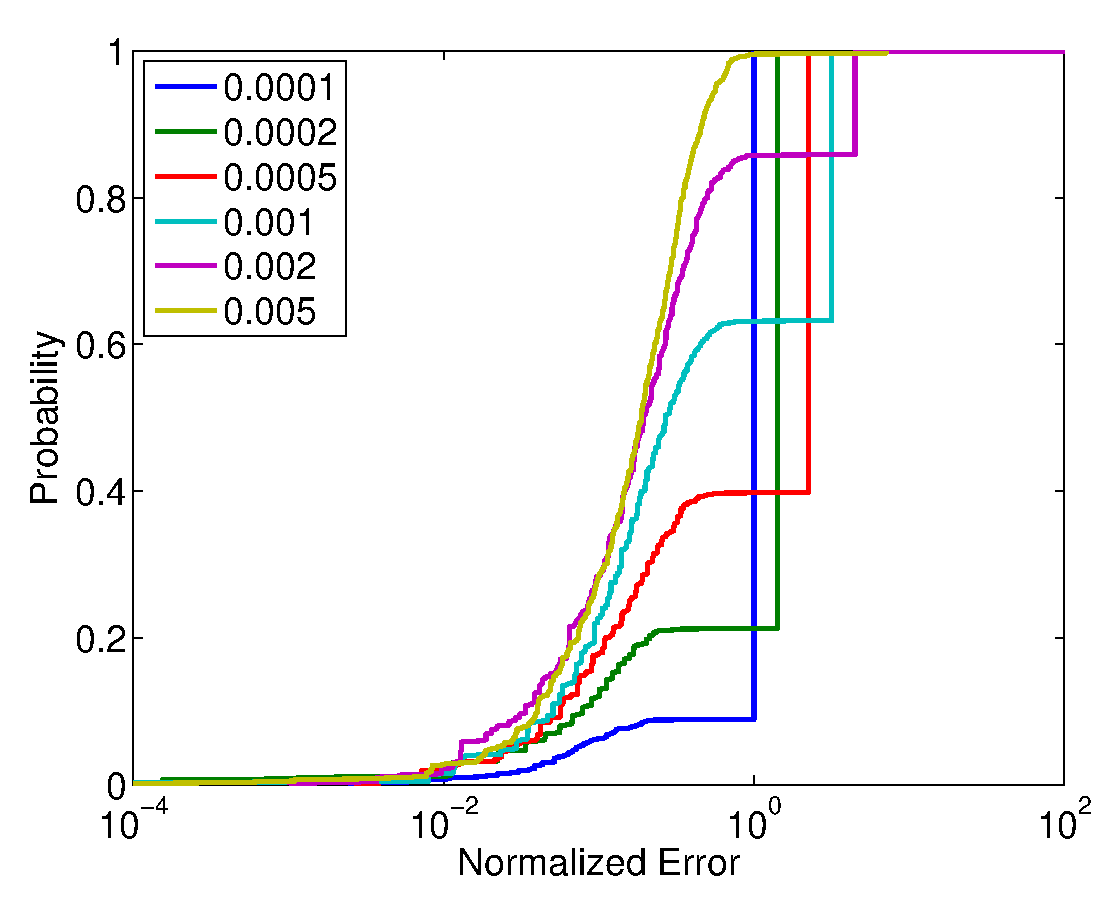
\includegraphics[width=3in]{NormalErrFig.eps}
\caption{Empirical distribution function of $\abs{\mu-\hmu_n}/0.01$ for example \eqref{exampleeq} and  various values of $p$ using the adaptive algorithm in Theorem \ref{mainadaptthm}. \label{normalerrfig}}
\end{figure}

The difficulty here is not a deficiency of the adaptive algorithm developed here, which is a modification of what is described above.  The point is that any algorithm can be fooled.  In this case, the initial sample used to estimate the variance of the integrand may miss a very narrow spike.  Without a good estimate of this variance, there is no reliable determination of the sample size needed for computing a sample mean that is close enough to the mean of the function.  Theorem \ref{mainadaptthm} describes under what conditions this adaptive algorithm will not be fooled.

The difficulties of error estimation are not unique to Monte Carlo methods. For the step function $f$ defined in \eqref{exampleeq}, MATLAB's {\tt quad} function approximates $\int_0^1 f(x - 1/\sqrt{2} \pmod 1) \, \dif x$  with an error tolerance of $10^{-14}$ to be $\approx 0.92911$, instead of the true answer of $1$.  Thus, the step function can fool automatic quadrature routines.  Figure \ref{foolquadfig} displays the integrand
\[
f(x) = 1+\cos\left(8\pi\min\left(\max\left(\frac{x-0.27158}{0.45684},0\right),1\right)\right), \qquad \int_0^1 f(x) \, \dif x = 1.54316.
\]
Here the constants $0.27158$ and $0.45684$ are chosen to fool MATLAB's {\tt quad} function.  Applying {\tt quad} to approximate the above integral with an error tolerance of $10^{-14}$ gives the answer $2$, since all of the integrand values sampled by {\tt quad} are $2$.  Thus, {\tt quad} is fooled again, even though this integrand has continuous first derivative.  

\begin{figure}
\centering
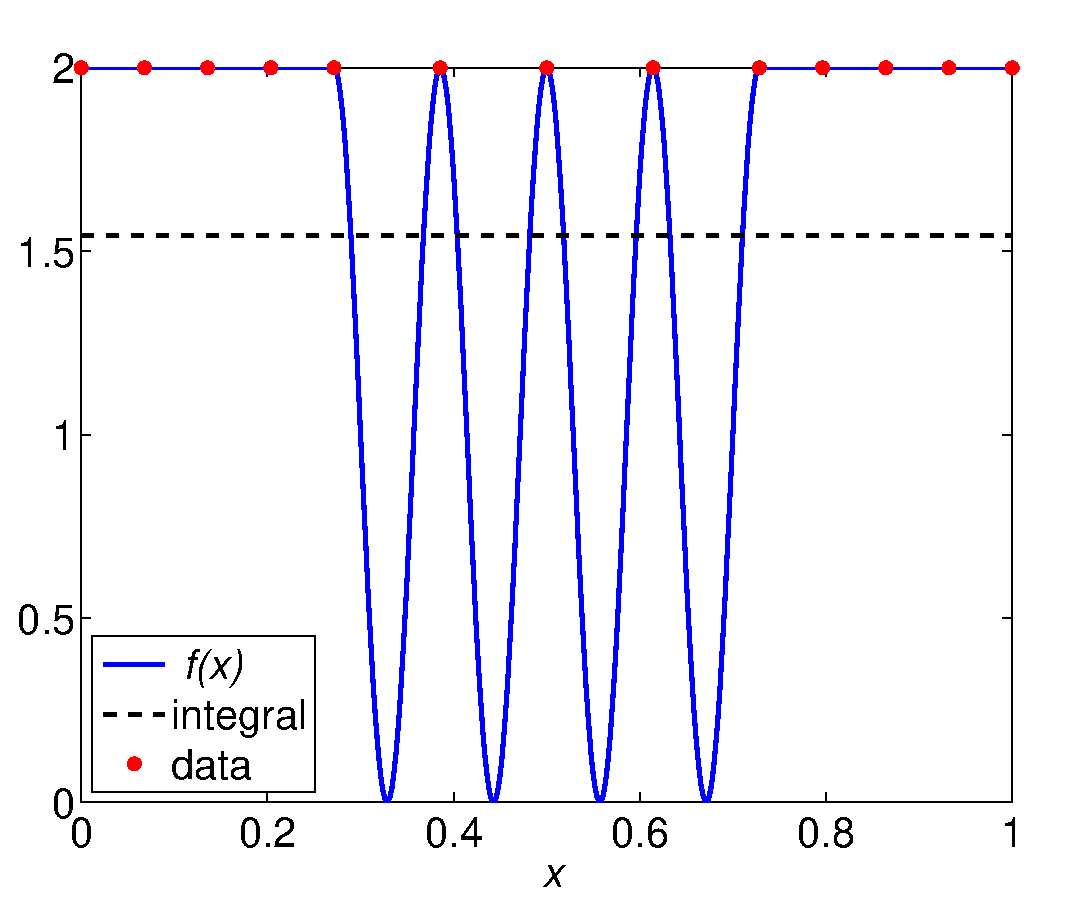
\includegraphics[width=3in]{FoolQuadFunction.eps}
\caption{Integrand that fools MATLAB's {\tt quad} function. \label{foolquadfig}}
\end{figure}

These two examples illustrate that although quadrature rules are valuable, they may give the wrong answers.  The goal of theory is to develop quadrature rules that have iron-clad sufficient conditions for the success.   This article does so for adaptive Monte Calo rules.  Thus, the step function example will be shown to fail to satisfy those conditions when the adaptive Monte Carlo rule fails to meet the required tolerance.

\section{Simple (I.I.D.) Monte Carlo with Guaranteed Error Estimation}

\subsection{Satisfying the Error Tolerance} First the question of bounding the variance is addressed.  The integrands under consideration are assumed to have finite moments of up to a order, $p$, i.e., a finite $\cl_{p}$ norm defined as follows:
\[
\norm[p]{f} :=\left\{\int_{\reals^d} \abs{f(\vx)}^p \rho(\vx) \, \dif \vx\right\}^{1/p}.
\]
The absolute centered $p^{\text{th}}$ moment of $f$ is defined as
\begin{equation} \label{momentdef}
M_p(f) := \int_{\reals^d} \abs{f(\vx)-\mu}^p \rho(\vx) \, \dif \vx = \norm[p]{f - \mu}^p, \qquad p \ge 1.
\end{equation}
By these definitions, the variance of $Y_1$ is the second moment, i.e., $M_2(f) = \var(Y_1)=\sigma^2$, and all functions in $\cl_2$ have finite variance.  Note that if $1 \le q \le p$, then by H\"older's inequality,
\begin{align*}\label{LP}
\norm[q]{f} &=\left\{\int_{\reals^d} \abs{f(\vx)}^q \rho(\vx) \, \dif \vx\right\}^{1/q}\\
\nonumber & \le \left\{\int_{\reals^d} \abs{f(\vx)}^p \, \rho(\vx) \, \dif \vx \right\}^{1/p} \left\{\int_{\reals^d} 1^{p/(p-q)} \, \rho(\vx) \, \dif \vx\right\}^{(p-q)/(pq)} = \norm[p]{f}.
\end{align*}
Thus, the $\cl_p$ norms and $M_p$ moments are related as follows:  
\begin{equation} \label{clinclude}
\norm[q]{f} \le \norm[p]{f}, \quad M_q(f) \le [M_p(f)]^{q/p}, \quad \cl_p \subseteq \cl_q \qquad \text{for } 1 \le q \le p .
\end{equation}


As mentioned in \eqref{samplevar}, a practical upper bound on this variance is obtained from the sample variance, $\hsigma^2 = \fudge^2 \hv_{n_{\sigma}}$, where $\fudge > 1$ is some variance inflation factor. This can be justified in a probabilistic sense by appealing to  Cantelli's inequality (Theorem \ref{Can}) and the variance of $\hv_{n_{\sigma}}$ given by Theorem \ref{Varvarthm}.  Proposition \ref{propCant} implies that
\[
\Prob \left[\frac{\hv_{n_{\sigma}}}{1 - \sqrt{\left ( \kappa  - \frac{n_{\sigma}-3}{n_{\sigma}-1}\right)\left(\frac{1-\alpha}{\alpha n_{\sigma}}\right)}} > \sigma^2 \right] \ge 1 - \alpha,
\]
where $\kappa$ is the \emph{kurtosis} of the integrand, defined as
\begin{equation} \label{kurtdef}
\kappa:= \kurt(f) = \frac{M_4(f)}{\var^2(f)} = \frac{M_4(f)}{\sigma^4} = \frac{M_4(f)}{M_2^2(f)} \ge 1 \qquad \forall f \in \cl_4.
\end{equation}
Note that the kurtosis of a function is independent of its scale, i.e., $\kurt(cf)=\kurt(f)$ for any $c \ne 0$.  Moreover, functions in $\cl_4$ automatically have finite variance.  It follows that the kurtosis of the integrand must be small enough, relative to $n_{\sigma}$ and $\fudge$ to ensure that the variance estimate is correct in a probabilistic sense, namely, 
\begin{multline}
\frac{1}{1 - \sqrt{\left ( \kappa  - \frac{n_{\sigma}-3}{n_{\sigma}-1}\right)\left(\frac{1-\alpha}{\alpha n_{\sigma}}\right)}} \le \fudge^2
\\
\iff \kappa \le \frac{n_{\sigma}-3}{n_{\sigma}-1} + \left(\frac{ \alpha n_{\sigma}}{1-\alpha}\right) \left(1 - \frac{1}{\fudge^2}\right)^2 =: \kappa_{\max} (\alpha,n_{\sigma},\fudge). \label{kappamaxdef}
\end{multline}

Figure \ref{kurtmaxcompareNfig}a shows how large a kurtosis can be accommodated for a given $n_{\sigma}$, $\alpha$, and variance inflation factor $\fudge=1.5$.  Note that for $n=30$, a common rule of thumb for applying the central limit theorem, even $\alpha=0.1$ gives $\kappa_{\max}$ of only about $2$, which is rather restrictive.

\begin{figure}
\centering
\begin{minipage}{2.1in}
\centering 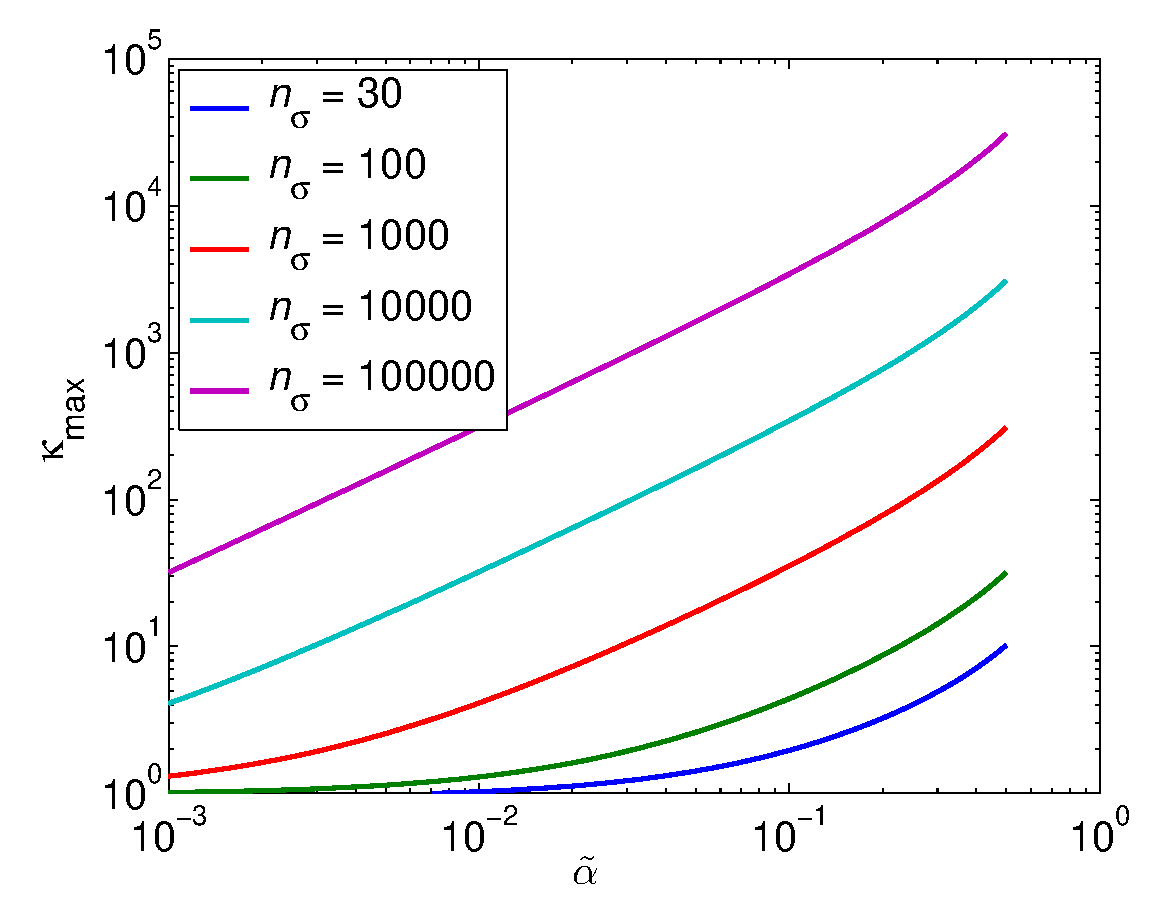
\includegraphics[width=2.1in]{kurtmaxfig.eps} \\
(a)
\end{minipage}
\quad 
\begin{minipage}{2.1in}\centering
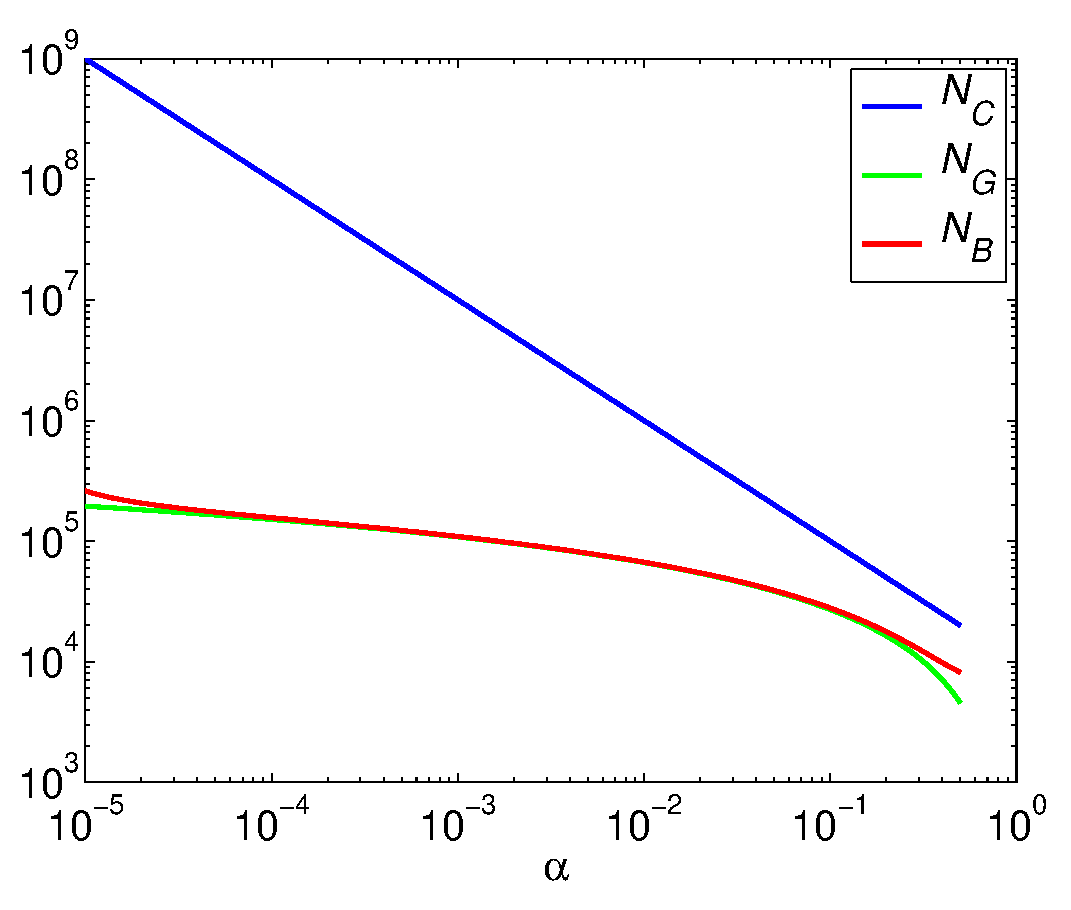
\includegraphics[width=2.1in]{alphacompare.eps}\\
(b)
\end{minipage}
\caption{(a) The maximum kurtosis, $\kappa_{\max}(\alpha,n_{\sigma},1.5)$, as defined in \eqref{kappamaxdef}; (b) comparison of sample sizes $ N_G(0.01,\alpha)$, $N_C(0.01,\alpha)$, and $N_B(0.01,\alpha,\kappa_{\max}^{3/4}(\alpha,1000,1.5))$.\label{kurtmaxcompareNfig}}
\end{figure}

The other issue that needs to be addressed is a tight probabilistic error bound.  The error bound given by the Central Limit Theorem, \eqref{CLT}, is only approximate.   Chebyshev's inequality implies that the number of function evaluations needed to ensure that $\hmu_n$ satisfies the error tolerance with high probability is
\begin{subequations} \label{ChebErr}
\begin{gather} \label{ChebProbEst}
\Prob\left[\abs{\hmu_n-\mu} \le \varepsilon \right] \ge 1-\alpha \quad \text{for } n \ge N_{C}(\varepsilon/\sigma,\alpha),\ f \in \cl_2,
\intertext{where }
\label{NCdef}
N_{C}(\varepsilon,\alpha) :=\left \lceil \frac{1}{\alpha\varepsilon^2} \right \rceil.
\end{gather}
\end{subequations}
However, this sample size is much larger than that given by the Central Limit Theorem, as shown in Figure \ref{kurtmaxcompareNfig}b.

Since higher order moments of the integrand are required to guarantee an upper bound on the true variance in terms of the sample variance, it is sensible to use these higher order moments to obtain smaller sample sizes.  A smaller sample size than \eqref{NCdef} with a rigorous probabilistic bound can be
found by invoking the non-uniform Berry-Esseen inequality (Theorem
\ref{BE}). This inequality makes strong assumptions on the
distribution of $f(\vX)$, namely, a finite third moment, $M_3 < \infty$.
Recalling that $Y_i = f(\vX_i)$, $\mu=E(Y_i)$, and $\hmu_n =
(Y_1 + \cdots + Y_n)/n$, it then follows by the non-uniform
Berry-Esseen inequality, that
\begin{align} 
\nonumber
\Prob\left[\abs{\hmu_n - \mu} <\frac{\sigma}{\sqrt{n}}x\right]&=\Prob\left[\hmu_n - \mu<\frac{\sigma}{\sqrt{n}}x\right]-\Prob\left[\hmu_n - \mu <-\frac{\sigma}{\sqrt{n}}x\right]\\
\nonumber
&\ge \left[\Phi(x)-\frac{0.56\widetilde{M}_3}{\sqrt{n}}(1+\abs{x})^{-3}\right] -\left[\Phi(-x) + \frac{0.56\widetilde{M}_3}{\sqrt{n}}(1+\abs{x})^{-3}\right]\\
&=1-2\left(\frac{0.56\widetilde{M}_3}{\sqrt{n}}(1+\abs{x})^{-3}+\Phi(-x)\right), \label{BEresult}
\end{align}
where $\widetilde{M}_3:=M_3/\sigma^3$, and $\Phi$ is the standard Gaussian cumulative distribution function.  Letting $x=\varepsilon\sqrt{n}/\sigma$, the probability of
making an error less than $\varepsilon$ is bounded below by $1-\alpha$, i.e., 
\begin{subequations} \label{proberrcritsampleBE}
\begin{equation}
\Prob[\abs{\hmu_n -\mu}<\varepsilon] \geq 1-\alpha,  \quad \text{provided } n \ge N_B(\varepsilon/\sigma,\alpha,\widetilde{M}_3), \ f \in \cl_3,
\end{equation}
where 
\begin{equation}\label{NB}
N_B(b,\alpha,M) := \min \left \{ n \in \naturals : \Phi\left(-b \sqrt{n}  \right)+\frac{0.56M}{\sqrt{n}\left(1+ b\sqrt{n} \right)^{3}}
\le \frac{\alpha}{2} \right \}.
\end{equation}
\end{subequations}

As shown in Figure \ref{kurtmaxcompareNfig}b, $N_B$ is quite close to $ N_G$ for a range of $\alpha$, but $N_B$ may be somewhat larger for very small or rather $\alpha$.  In general $N_B$ is smaller than $N_C$, but not always.  A disadvantage of \eqref{proberrcritsampleBE} is that class of integrands, $\cl_3$, is smaller than that in \eqref{ChebErr}, but this typically a small price to pay given the much smaller cost of computation.

The theorem below combines the results on estimating the variance with the sample sizes arising from Chebyshev's inequality and the Berry-Esseen inequality.  These lead to an adaptive Monte Carlo algorithm with a probabilistic error guarantee.

\begin{theorem} \label{mainadaptthm} Specify the following parameters defining the algorithm:
\begin{itemize}
\item sample size for variance estimation, $n_{\sigma} \in \naturals$,
\item variance inflation factor for variance estimation, $\fudge \in (1,\infty)$,
\item uncertainty tolerance, $\alpha\in (0,1)$, and $\talpha = 1 - \sqrt{1 - \alpha}$, and
\item relative error tolerance, $\varepsilon \in (0,1)$. 
\end{itemize} 
Define the set of functions with bounded kurtosis:
\[
\cf^{\kurt}= \{f \in \cl_{4} : \kurt(f)= \kappa \le \kappa_{\max}(n_{\sigma},\talpha,\fudge) \},
\]
where $\kappa_{\max}$ is defined in \eqref{kappamaxdef}.  For any $f \in \cf^{\kurt}$, compute the sample variance, $\hv_{n_{\sigma}}$ using a simple random sample of size $n_{\sigma}$. Use this to approximate the variance of $f$ by $\hsigma^2 = \fudge^2 \hv_{n_{\sigma}}$ as in \eqref{sigmadef}.  Next define a sample size
\[
n = N_{CB}(\varepsilon/\hsigma,\talpha,\kappa_{\max}^{3/4}),
\]
where
\begin{equation} \label{NCBdef}
N_{CB}(b,\alpha,M) := \min\left( N_C(b,\alpha), N_B(b,\alpha,M) \right),
\end{equation} 
$N_C$ is defined in \eqref{NCdef} and  $N_B$ is defined in \eqref{NB}.  Compute $\hmu_n$, the simple Monte Carlo estimator of $\mu$ based on $n$ samples, as in \eqref{simpleMCest}.  A probabilistic absolute error bound is given by
\[
\Prob\left[\abs{\hmu_n-\mu} \le \varepsilon \right] \geq 1-\alpha.
\]
\end{theorem}
\begin{proof} Note that \eqref{clinclude} implies that the third moment can be bounded in terms of the fourth moment, namely $\widetilde{M}_3 \le \kappa^{3/4}$. There are three primary random variables in this algorithm:  the estimated upper bound on the standard deviation, $\hsigma$, the sample size to estimate the mean, $n$, which is an explicit function of $\hsigma$, and the estimated mean, $\hmu_n$. By  \eqref{ChebErr} and \eqref{proberrcritsampleBE} it then follows that  $\Prob\left[\abs{\hmu_n-\mu} \le \varepsilon \right] \geq 1-\talpha$, provided that $\hsigma  \ge \sigma$. Thus, 
\begin{align*}
\Prob\left[\abs{\hmu_n-\mu} \le \varepsilon \right] &
= E_{\hsigma} \left\{\Prob\left[\abs{\hmu_n-\mu} \le \varepsilon \ | \ \hsigma \right] \right\} \\
& \ge E_{\hsigma} \left\{(1-\talpha) 1_{[\sigma,\infty)}(\hsigma) \right\}\\
& \ge (1-\talpha) (1-\talpha) = 1-\alpha,
\end{align*}
since $\hsigma \ge \sigma$ with probability $1-\talpha$ by \eqref{kappamaxdef}.  \qed
\end{proof}

\subsection{Cost of the Algorithm}  The sample size of the adaptive algorithm defined in Theorem \ref{mainadaptthm} is a random variable, and so the cost of this algorithm might best be defined defined probabilistically.  Moreover, the cost depends strongly on the $\sigma$ as well as the $\varepsilon$, and its definition should reflect this dependence. 

Let $A$ be any random algorithm defined for a set of integrands $\cf$ that takes as its input an error tolerance, $\varepsilon$, an uncertainty level, $\alpha$, and a  procedure for computing values of $f \in \cf$.  The algorithm then computes an approximation to the integral, $A(f,\varepsilon,\alpha)$, satisfying a probabilistic error criterion,
\[
\Prob[\abs{\mu - A(f,\varepsilon,\alpha)} < \varepsilon] \le 1 - \alpha,
\]
The integral approximation, $A(f,\varepsilon,\alpha)$ is based solely on  $f(\vx_1), \ldots, f(\vx_n)$, where the choice of each $\vx_i$ may depend iteratively on $(\vx_1,f(\vx_1)), \ldots, (\vx_{i-1},f(\vx_{i-1}))$, and the decision to stop with $n$ data depends on all function data collected up to and including the $n^{\text{th}}$.  Then $\card(A,\varepsilon,\alpha,f):=n$, which as noted is a random variable.  The probabilistic cost of the algorithm, with uncertainty $\beta$, for integrands of variance no greater than $\sigma^2$ is defined as 
\begin{equation}
\cost(A,\varepsilon,\alpha,\beta,\cf,\sigma) := \sup_{\substack{f \in \cf\\ \var(f)\le \sigma^2} } \min\left\{M : \Prob[\card(A,\varepsilon,\alpha,f) \le M] \ge 1-\beta  \right \}.
\end{equation}

The cost of the particular adaptive Monte Carlo algorithm defined in Theorem \ref{mainadaptthm}, denoted $\aMC$, for the class of functions $\cf^{\kurt}$ is
\begin{equation}
\cost(\aMC,\varepsilon,\alpha, \beta, \cf^{\kurt}, \sigma) := \sup_{\substack{f \in \cf^{\kurt}\\ \var(f)\le \sigma^2} } \min\left\{M : \Prob(n_{\sigma} + n \le M) \ge 1-\beta  \right \}.
\end{equation}
Since $n_{\sigma}$ is fixed, bounding this cost depends on bounding $n$, which depends on $\hsigma$ as given by Theorem \ref{mainadaptthm}.  Moreover, $\hsigma$ can be bounded using Proposition \ref{propCant}:
\begin{align*}
1-\beta & \le \Prob\left[\hv_{n_{\sigma}} < \sigma^2 \left\{1 + \sqrt{\left ( \kappa  - \frac{n_{\sigma}-3}{n_{\sigma}-1}\right)\left(\frac{1-\beta}{\beta n_{\sigma}}\right)}\right\} \right] \\
& \le \Prob\left[\hsigma^2 = \fudge^2 \hv_{n_{\sigma}} < \fudge^2\sigma^2 \left\{1 + \sqrt{\left ( \kappa_{\max}(n_{\sigma},\talpha,\fudge)  - \frac{n_{\sigma}-3}{n_{\sigma}-1}\right)\left(\frac{1-\beta}{\beta n_{\sigma}}\right)}\right\} \right] \\
%& = \Prob\left[\hsigma^2 < \fudge^2\sigma^2 \left\{1 + \sqrt{\left(\frac{ \talpha }{1-\talpha}\right) \left(\frac{1-\beta}{\beta}\right) \left(1 - \frac{1}{\fudge^2}\right)^2}\right\} \right] \\
& = \Prob\left[\hsigma^2 < \sigma^2 \gamma^2(\talpha,\beta,\fudge) \right],
\end{align*}
where
\[
\gamma^2(\talpha,\beta,\fudge) := \fudge^2 \left\{1 + \sqrt{\left(\frac{ \talpha }{1-\talpha}\right) \left(\frac{1-\beta}{\beta}\right) \left(1 - \frac{1}{\fudge^2}\right)^2}\right\} > 1.
\]
Noting that $N_{CB}(\cdot,\alpha,M)$ is a non-increasing function allows one to derive the following upper bound on the cost of the adaptive Monte Carlo algorithm.

\begin{theorem} \label{costtheorem} The adaptive Monte Carlo algorithm described in Theorem \ref{mainadaptthm}, denoted $\aMC$, has a probabilistic cost bounded above by 
\begin{equation*}
\cost(\aMC,\varepsilon,\alpha, \beta, \cf^{\kurt}, \sigma)
\le n_{\sigma} + N_{CB}(\varepsilon/(\sigma\gamma(\talpha,\beta,\fudge)),\talpha,\kappa_{\max}^{3/4}).
\end{equation*} 
\end{theorem}

The cost of the adaptive Monte Carlo algorithm $\aMC$ is roughly proportional to $\sigma^2\varepsilon^{-2}$.  The set $\cf^{\kurt}$ contains integrands with arbitrarily large variance, $\sigma^2$ and thus with potentially arbitrarily large algorithmic cost.  On the other hand, the cost does seem to depend on the integrand variance as expected.  The variable cost of the algorithm for integrands in $\cf^{\kurt}$ is actually an advantage, rather than a drawback, of this analysis.  One need not make any a priori assumptions about the size of the integrand, $\sigma$, only about the kurtosis, $\kappa$, which is unchanged when the integrand is multiplied by an arbitrary nonzero constant.

Whereas $\sigma$ can be thought of as the size of the integrand, the kurtosis is a measure of the integrands \emph{nastiness}.  The larger the kurtosis, the more difficult it is to estimate $\sigma$, and thus choose the proper sample size to obtain the desired error tolerance.

\section{Simple Monte Carlo Satisfying a Relative Error Criterion} \label{relerrsec}

In many practical situations, one needs to approximate the integral with a certain relative accuracy.  For example, one wants an answer that is correct to three significant digits.  In this case, given a tolerance, $\varepsilon$, and a significance level $\alpha$, with $\varepsilon, \alpha \in (0, 1)$, one seeks a random $\tmu$ such that 
\begin{equation} \label{relerrcrit}
\Prob\left[\abs{\frac{\tmu-\mu}{\mu}} \le \varepsilon \right] \geq 1-\alpha.
\end{equation}
Clearly, one must have $\mu\ne0$ for such a statement to be possible.  Using straightforward algebraic manipulations, this condition may be written equivalently as 
\begin{equation} \label{relerrcritb}
\Prob\left[\frac{\tmu}{1 + \varepsilon \sign(\mu)} \le \mu \le \frac{\tmu}{1 - \varepsilon \sign(\mu)} \right] \geq 1-\alpha.
\end{equation}
The above form is not a traditional confidence interval, however, suppose that one has the following confidence interval for $\mu$ in terms of $\hmu$ and $\tvareps$: 
\begin{equation} \label{relerrcritc}
1-\alpha \le \Prob\left[\abs{\hmu-\mu} \le \tvareps \right] = \Prob\left[\hmu -\tvareps \le \mu \le \hmu + \tvareps \right], \quad \text{with} \quad 0 < \tvareps/\abs{\hmu} \le \varepsilon.
\end{equation}
Letting $\tmu = \hmu(1 - \tvareps^2/\hmu^2)$, it follows that 
\begin{align*} 
1-\alpha &\le \Prob\left[\hmu -\tvareps \le \mu \le \hmu + \tvareps \right] =\Prob\left[\frac{\tmu}{1+\tvareps/\hmu} \le \mu \le \frac{\tmu}{1-\tvareps/\hmu} \right] \\
&\le\Prob\left[\frac{\tmu}{1+\varepsilon\sign(\hmu)} \le \mu \le \frac{\tmu}{1-\varepsilon\sign(\hmu)} \right]
\end{align*}
Since \eqref{relerrcritc} implies that $\sign(\mu) = \sign(\hmu)$, the relative error criterion \eqref{relerrcritb}, and thus \eqref{relerrcrit}, are satisfied.  The previous section shows how to find absolute error criteria of the form \eqref{relerrcritc}, but the challenge is to ensure that $\tvareps \le \varepsilon\abs{\hmu}$ when $\hmu$ is not known in advance.  This is done iteratively as described in Theorem \ref{relerradaptthm} below.

Some notation is needed for this theorem.  For any fixed $\alpha \in (0,1)$, and $M>0$, define the inverse of the functions $N_C(\cdot,\alpha)$, $N_B(\cdot,\alpha,M)$, and $N_{CB}(\cdot,\alpha,M)$,
\begin{subequations} \label{probadapterrcritBE}
\begin{gather}\label{NCinv}
N_C^{-1}(n,\alpha) := \frac{1}{\sqrt{n \alpha}}, \\
\label{NBinv}
N_B^{-1}(n,\alpha,M) := \min \left \{ b>0 : \Phi\left(-b \sqrt{n}  \right)+\frac{0.56M}{\sqrt{n}\left(1+ b\sqrt{n} \right)^{3}}
\le \frac{\alpha}{2} \right \}, \\
\label{NCBinv}
N_{CB}^{-1}(n,\alpha,M) := \min(N_C^{-1}(n,\alpha),N_B^{-1}(n,\alpha,M)).
\end{gather}
It then follows then by Chebyshev's inequality and the Berry-Esseen Inequality (see Theorem \ref{BE} and \eqref{BEresult}) that 
\begin{equation}
\Prob[\abs{\hmu_n -\mu}<\tvareps] \geq 1-\alpha, \quad \text{provided } \ f \in \cl_3, \qquad \text{where }\tvareps=\sigma N_{CB}^{-1}(n,\alpha,\widetilde{M}_3), 
\end{equation} 
\end{subequations}
and $\widetilde{M}_3$ is the scaled absolute third moment of the integrand.  Given a significance level, $\alpha \in (0,1)$, let $\alpha_{\sigma}, \alpha_1,  \alpha_2, \ldots$ be an infinite sequence of positive numbers such that 
\begin{equation} \label{alphaseq}
(1-\alpha_{\sigma})(1-\alpha_1)(1-\alpha_2) \cdots = 1-\alpha.
\end{equation}
Fore example, one might choose
\begin{equation} \label{alphaseqex}
\alpha_{\sigma} = 1-\me^{-b}, \ \ \alpha_{i} = 1-\me^{-ba^{-i}}, \ i\in \naturals, \quad \text{where} \  a \in (1,\infty), \  b=\frac{1-a}{a} \log(1-\alpha).
\end{equation}

\begin{theorem} \label{relerradaptthm} Specify the following parameters defining the algorithm:
\begin{itemize}
\item sample size for variance estimation, $n_{\sigma} \in \naturals$,
\item initial sample size for mean estimation, $n_1 \in \naturals$,
\item variance inflation factor for variance estimation, $\fudge \in (1,\infty)$, 
\item factor for confidence interval width reduction, $\delta \in (0,1)$,
\item uncertainty tolerance, $\alpha\in (0,1)$, and a sequence $\alpha_{\sigma}, \alpha_1,  \alpha_2, \ldots$ satisfying \eqref{alphaseq}, and
\item relative error tolerance, $\varepsilon \in (0,1)$. 
\end{itemize} 
Define the set of functions with bounded kurtosis and nonzero mean:
\[
\cf^{\kurt}_0= \{f \in \cl_{4} : \kurt(f)= \kappa \le \kappa_{\max}(n_{\sigma},\alpha_{\sigma},\fudge), \mu(f) \ne 0\},
\]
where $\kappa_{\max}$ is defined in \eqref{kappamaxdef}.  For any $f \in \cf^{\kurt}_0$, compute the sample variance, $\hv_{n_{\sigma}}$ using a simple random sample of size $n_{\sigma}$. Use this to approximate the variance of $f$ by $\hsigma^2 = \fudge^2 \hv_{n_{\sigma}}$, as in \eqref{sigmadef}, and to compute the width of initial the confidence interval for the mean, $\tvareps_1=\hsigma N_{CB}^{-1}(n_1,\alpha_1,\kappa_{\max}^{3/4})$.  For $i=1, 2, \ldots$, do the following:
\begin{enumerate}
\renewcommand{\labelenumi}{\alph{enumi})}
\item Compute the sample average $\hmu_{n_i}$ using a simple random sample that is independent of those used to compute $\hv_{n_{\sigma}}$ and $\hmu_{n_1}, \ldots, \hmu_{n_{i-1}}$.

\item If $\tvareps_i > \varepsilon \abs{\hmu_{n_i}}$, then reduce the width of the next confidence interval for the mean, 
\[
\tvareps_{i+1} = \min(\delta\tvareps_i, \varepsilon \max(\tvareps_i,\abs{\hmu_{n_i}}-\tvareps_i)).
\]
Define the next sample size, $n_{i+1} = N_{CB}(\tvareps_{i+1}/\hsigma,\alpha_{i+1},\kappa_{\max}^{3/4})$,
increase $i$ by one, and go to step a). 

\item Else, let $\tmu = \hmu_{n_i}(1 - \tvareps_i^2/\hmu_{n_i}^2)$, and terminate the algorithm because the relative error criterion, \eqref{relerrcrit}, is satisfied.

\end{enumerate}
\end{theorem}

\begin{proof} In this algorithm there are a number of important random variables:  the estimated upper bound on the standard deviation, $\hsigma$, the sample sizes $n_1, \ldots, n_\tau$, the number of confidence intervals computed, $\tau$, and the estimates of the mean, $\hmu_{n_1}, \ldots, \hmu_{n_{\tau}}$. These sample means are conditionally independent given the sequence of sample sizes.  The probability that the final confidence interval is correct, is then no less than the probability that all of the confidence intervals are correct, conditioned on the sample sizes.  Specifically,
\begin{align*}
\Prob\left[\abs{\frac{\tmu-\mu}{\mu}} \le \varepsilon \right] & 
\ge \Prob\left[\abs{\hmu_{n_{\tau}}-\mu} \le \tvareps_{n_{\tau}} \ \& \ \varepsilon \hmu_{n_{\tau}} \le \tvareps_{n_{\tau}} \right] \\
& = E \left\{\Prob\left[\abs{\hmu_{n_{\tau}}-\mu} \le \tvareps_{n_{\tau}} \ \& \ \varepsilon \hmu_{n_{\tau}} \le \tvareps_{n_{\tau}} \ | \ \hsigma, \tau, n_1, \ldots, n_{\tau} \right] \right\} \\
& \ge E \left\{\Prob\left[\abs{\hmu_{n_{i}}-\mu} \le \tvareps_{n_{i}}] \forall i \ \& \ \varepsilon \hmu_{n_{\tau}} \le \tvareps_{n_{\tau}} \ | \ \hsigma, \tau, n_1, \ldots, n_{\tau} \right] \right\} \\
& \ge E_{\hsigma} \left\{[(1-\alpha_1)(1-\alpha_2) \cdots] 1_{[\sigma,\infty)}(\hsigma) \right\}\\
& \ge (1-\alpha_{\sigma}) (1-\alpha_1)(1-\alpha_2) \cdots = 1-\alpha. \qquad \qed
\end{align*}
\end{proof}


\section{Numerical Examples}


\section{Questions}

Here are some questions that suggest themselves:

\begin{itemize}

\item Can this type of analysis be extended to randomized \emph{quasi-Monte Carlo} for finite dimension, $d$?  Infinite dimension?  In this latter case one needs some multilevel algorithm, but the specification of the levels perhaps could be deduced from the data.  One might also consider a case where the coordinate weights were not known a priori but needed to be estimated.

\item Is there already this kind of information-based complexity analysis where the number of operations is bounded above or below by the unknown scale of the problem (in this case the variance).  The IBC I know assumes that the scale is fixed, e.g., the function has variance one, norm one, etc.  Here we allow arbitrary scale, but do make assumptions on the nastiness (kurtosis).

\item Are there better inequalities than Chebyshev's inequality or the Berry-Esseen inequality that apply when $Z$ is the sum of i.i.d.\ random variables?  Some of the better known ones, like Hoeffding's inequality assume boundedness, which we cannot presume here.

\end{itemize}

\section{Appendix of Useful Results}
\begin{theorem}[Chebyshev's Inequality] \label{Chebineqthm} Let $Z$ be any random variable with mean $\mu$ and variance $\sigma^2$.  Then for all $\alpha >0$,
\[
\Prob\left[\abs{Z-\mu} \ge \frac{\sigma}{\sqrt{\alpha}} \right] \le \alpha, \qquad \Prob\left[\abs{Z-\mu} < \frac{\sigma}{\sqrt{\alpha}} \right] \ge 1-\alpha.
\]
\end{theorem}
\begin{proof}To prove Chebyshev's inequality note that
\begin{equation*}
\sigma^2 = E[\abs{Z-\mu}^2] \ge \frac{\sigma^2}{\alpha} \Prob\left[\abs{Z-\mu} \ge \frac{\sigma}{\sqrt{\alpha}} \right],
\end{equation*}
and then divide both sides by $\sigma^2/\alpha$. \qed
\end{proof}
\begin{theorem}[Non-uniform Berry-Esseen Inequality] \cite[Theorem 5.16, p. 168]{Pet95a} \label{BE} Let $Y_1,\dots,Y_n$ be i.i.d.\ random variables.  Suppose that
$\mu=E(Y_i)$, $\var(Y_i)=\sigma^2>0$,  and $\widetilde{M}_3=E\abs{Y_i - \mu}^3/\sigma^3 < \infty$.
Then
\[
\abs{\Prob\left[\frac{1}{\sigma\sqrt{n}}\sum_{i=1}^{n}(Y_i-\mu)<x
\right]-\Phi(x)}\leq \frac{A \widetilde{M}_3}{\sqrt{n}}(1+\abs{x})^{-3}.
\] for all x,
where $\Phi$ is the cumulative distribution function of the standard normal random variable, and $A$ is some number satisfying $0.4097\leq A\leq 0.5600$.
\end{theorem}

\begin{theorem} \label{Varvarthm} Let $Y_1, Y_2, \ldots$ be i.i.d.\ random variables,  $\hmu_n$ be the sample mean as defined in \eqref{samplemean}, and $\hv_n$ be the sample variance as defined in \eqref{samplevar}.  Then the variance of the sample variance and the kurtosis of the sample mean are given by 
\[
\var(\hv_n^2) = \frac{\sigma^4}{n} \left ( \kappa  - \frac{n-3}{n-1} \right), \qquad \kurt(\hmu_n) = \frac{\kappa + 3(n-1)}{n} = \frac{(\kappa -3)}{n} + 3
\]
where $\kappa$ is the kurtosis of $Y_1$.
\end{theorem}
\begin{proof} Without loss of generality, it may be assumed that the $Y_i$ have zero mean.  If they do not, the mean may be subtracted off. The sample variance and its square may be written in terms of multiple sums of the $Y_i$ as follows:
\begin{align*}
\hv_n & =  \frac 1{n-1} \sum_{i=1}^n \left[Y_i- \left(\frac 1n \sum_{j=1}^n Y_j\right) \right]^2
=  \frac 1{n(n-1)}\left[ n \sum_{i=1}^n Y^2_i-  \sum_{j,k=1}^n Y_jY_k \right] \\
\hv_n^2 & = \frac 1{n^2(n-1)^2}\left[ n^2 \sum_{i,j=1}^n Y^2_i Y^2_j  - 2 n \sum_{i,j,k=1}^n Y^2_i Y_j Y_k +  \sum_{i,j,k,l=1}^n Y_iY_j Y_k Y_l\right].
\end{align*}
The expected values of each of these multiple sums can be computed in terms of $\sigma^2=E[Y_i^2]$ and $\kappa=E[Y_i^4]/\sigma^4$: 
\begin{align*}
E[ Y^2_i Y^2_j] & = \begin{cases} \kappa \sigma^4, & i=j,\\
\sigma^4, & i \ne j,
\end{cases} \qquad  
\sum_{i,j=1}^n E[Y^2_i Y^2_j] = n\sigma^4 (\kappa + n-1), \\
E[ Y^2_i Y_j Y_k] & = \begin{cases}  \kappa \sigma^4, & i=j=k,\\
\sigma^4, & i \ne j, j=k,\\
0, & j \ne k,
\end{cases}  \qquad  
\sum_{i,j,k=1}^n E[Y^2_i Y_j Y_k] = n\sigma^4 (\kappa + n-1) \\
E[ Y_i Y_j Y_k Y_l] & = \begin{cases} \kappa \sigma^4, & i=j=k=l,\\
\sigma^4, & i, j, k, l \text{ have two pairs of distinct values},\\
0, & \text{otherwise},
\end{cases}\\
\sum_{i,j,k,l=1}^n E[Y_iY_j Y_k Y_l] &= n\sigma^4[ \kappa + 3(n-1)]
\end{align*}
This last expectations yields the kurtosis of the sample mean:
\[
\kurt(\hmu_n) = \frac{E\left[ \left\{\frac{1}{n} \sum_{i=1}^n Y_i \right\}^4\right]}{[\var(\hmu_n)]^2} = \frac{n^{-4} E\left[ \sum_{i,j,k,l=1}^n Y_iY_j Y_k Y_l \right]}{\sigma^4/n^2} = \frac{\kappa + 3(n-1)}{n} 
\] 
Combining these expectations also yields the expected value for $\hv_n^2$ and the variance of $\hv_n$, since the sample variance has mean $\sigma^2/n$: 
\begin{align*}
E[\hv_n^2] & = \frac{ n^3\sigma^4 (\kappa + n-1)  - 2 n^2 \sigma^4(\kappa + n-1) +  n\sigma^4 [\kappa + 3(n-1)]} {n^2(n-1)^2} \\
& = \frac{\sigma^4[ (n-1)\kappa + (n^2-2n+3)]} {n(n-1)} \\
\var(\hv_n^2) & = E[\hv_n^2] - \left[E(\hv_n)\right]^2 = \sigma^4 \frac{ (n-1)\kappa + (n^2-2n+3)} {n(n-1)} -\sigma^4 = \frac{\sigma^4}{n} \left ( \kappa  - \frac{n-3}{n-1} \right).
\end{align*}
\hfill \hfill \qed
\end{proof}
\begin{theorem}[Single tailed Cantelli's inequality]\label{Can}
Let $Z$ be any random variable with mean $\mu$ and finite variance $\sigma^2$.  For any $a\geq 0$, it
follows that:
\[
\Prob[Z-\mu \geq a]\leq \frac{\sigma^2}{a^2+\sigma^2}.
\]
\end{theorem}
\begin{proof}Define the random variable
\[ S=\sign(Z - \mu - a) = \begin{cases} 1, & Z - \mu \geq a,\\ -1, & Z - \mu <a. \end{cases}
\]
From conditional probability it is known that
\begin{align*}
\sigma^2 &= \var(Z-\mu)=E[\var(Z-\mu|S)]+\var[E(Z-\mu|S)] \\
&\geq\var[E(Z-\mu|S)]= E[\{E(Z-\mu|S)\}^2]-[E\{E(Z-\mu|S)\}]^2 =  E[\{E(Z-\mu|S)\}^2]
\end{align*}
Since $E(Z-\mu)=0$, it follows that
\begin{equation*}
0= E[E(Z-\mu|S)]=E(X|S=1)\Prob(Z - \mu \geq a)+E(X|S=-1)\Prob(Z - \mu < a).
\end{equation*}
Also, it is clear that $E(Z - \mu|S=1) \ge a$, which implies that
\begin{equation*}
[E(Z - \mu|S=-1)]^2=\left[\frac{E(Z - \mu|S=1)\Prob(Z - \mu \geq a)}{\Prob(Z - \mu < a)}\right]^2\geq \left[\frac{a\Prob(Z - \mu \geq a)}{\Prob(Z - \mu < a)}\right]^2
\end{equation*}
Combining these results together yields
\begin{align*}
\sigma^2 & \ge E[\{E(Z-\mu|S)\}^2]\\
& =\{E(Z-\mu|S=1)\}^2 \Prob(Z - \mu \geq a) + \{E(Z-\mu|S=-1)\}^2 \Prob(Z - \mu < a) \\
& \ge a^2 \Prob(Z - \mu \geq a) + \left[\frac{a\Prob(Z - \mu \geq a)}{\Prob(Z - \mu < a)}\right]^2 \Prob(Z - \mu < a) \\
&= a^2 \left[\frac{ \Prob(Z - \mu \geq a)}{\Prob(Z - \mu < a)}\right] = a^2 \left[\frac{ \Prob(Z - \mu \geq a)}{1  - \Prob(Z - \mu \ge a)}\right]
\end{align*}
Solving this inequality for $\Prob(Z - \mu \geq a)$ completes the proof. \qed
\end{proof}

\begin{prop}\label{propCant} Let $\hv_n$ be the sample variance of a function $g$ as defined in \eqref{samplevar}, and let $\kappa=\kurt(g)$.  Then
\begin{subequations} \label{sampvarbd}
\begin{gather}\label{sampvarup}
\Prob\left[\hv_n < \sigma^2 \left\{1 + \sqrt{\left ( \kappa  - \frac{n-3}{n-1}\right)\left(\frac{1-\alpha}{\alpha n}\right)}\right\} \right] \ge 1 - \alpha, \\
\label{sampvarlo}
\Prob\left[\hv_n > \sigma^2 \left\{1 - \sqrt{\left ( \kappa  - \frac{n-3}{n-1}\right)\left(\frac{1-\alpha}{\alpha n}\right)}\right\} \right] \ge 1 - \alpha.
\end{gather}
\end{subequations}
\end{prop}
\begin{proof}Choosing
$$a=\sigma^2\sqrt{\left(\kappa-\frac{n-3}{n-1}\right)\left(\frac{1-\alpha}{\alpha n}\right)} >0,
$$
it follows from Cantelli's inequality (Theorem \ref{Can})  that
\begin{multline*}
\Prob\left[\hv_n-\sigma^2 \geq
\sigma^2\sqrt{\left(\kappa-\frac{n-3}{n-1}\right)\left(\frac{1-\alpha}{\alpha n}\right)} \right]  = \Prob\left[\hv_n-\sigma^2 \geq
a \right]\\
 \leq\frac{\var(\hv_n)}{a^2+\var(\hv_n)} 
= \frac{\frac{\sigma^4}{n}\left(\kappa - \frac{n-3}{n-1}\right)}{\frac{\sigma^4}{n}\left(\kappa - \frac{n-3}{n-1}\right)\left(\frac{1-\alpha}{\alpha}\right)+\frac{\sigma^4}{n}\left(\kappa - \frac{n-3}{n-1}\right)} 
=\frac{1}{\left(\frac{1-\alpha}{\alpha}\right)+1}=\alpha.
\end{multline*}
Then \eqref{sampvarup} follows directly.  By a similar argument, applying Cantelli's inequality to the expression $\Prob\left[-\hv_n+\sigma^2 \ge a \right]$ implies  \eqref{sampvarlo}. \qed
\end{proof}

\begin{prop}\label{latnetprop} For the situation described in Section \ref{qmcsec} with the operations $\oplus$, $\ominus$, and $\otimes$, the basis functions $\phi_{\vk}$, and any $\oplus$-closed set, $P$, with cardinality $\abs{P}$ and associated dual lattice $P^{\perp}$, it follows that 
\begin{gather}
\label{basisorth}
\mu(\phi_{\vk})= \int_{\cube} \phi_{\vk}(\vx) \, \dif \vx = \int_{\cube} e^{2 \pi \sqrt{-1} \vk \otimes \vx} \, \dif \vx = \delta_{\vk, \vzero}, \\
\label{duallatorth}
Q(\phi_{\vk},P,\vDelta)= \frac{1}{\abs{P}}\sum_{\vx \in P} \phi_{\vk}(\vx \oplus \vDelta) = \begin{cases} \phi_{\vk}(\vDelta), & \vk \in P^{\perp} \\ 0, & \vk \notin P^{\perp}
\end{cases}
\end{gather}
\end{prop}
\begin{proof}
The properties assumed for the binary operations imply that for all $\vt \in \cube$,
\begin{align*}
\int_{\cube} \phi_{\vk}(\vx) \, \dif \vx &= \int_{\cube} \phi_{\vk}(\vx \oplus \vt) \, \dif \vx = \phi_{\vk}(\vt) \int_{\cube} \phi_{\vk}(\vx) \, \dif \vx\\
0 & = \left [\phi_{\vk}(\vt) -1 \right] \int_{\cube} \phi_{\vk}(\vx) \, \dif \vx
\end{align*}
This inequality is satisfied iff $\vk=\vzero$ or $\int_{\cube} \phi_{\vk}(\vx) \, \dif \vx =0$.  This establishes \eqref{basisorth}. 

A similar argument establishes \eqref{duallatorth}.  Note first that the sum can be simplified to a multiple of $\phi_{\vk}(\vDelta)$:
\begin{equation*}
\frac{1}{\abs{P}}\sum_{\vx \in P} \phi_{\vk}(\vx \oplus \vDelta) 
= \frac{1}{\abs{P}}\sum_{\vx \in P} [\phi_{\vk}(\vx) \phi_{\vk}(\vDelta)] = \phi_{\vk}(\vDelta) \frac{1}{\abs{P}}\sum_{\vx \in P} \phi_{\vk}(\vx).
\end{equation*}
Next, note that for all $\vt \in P$ the remaining sum above is unchanged when the argument of $\phi_{\vk}$ is shifted by $\vt$:
\begin{align*}
\frac{1}{\abs{P}}\sum_{\vx \in P} \phi_{\vk}(\vx) 
& = \frac{1}{\abs{P}}\sum_{\vx \in P} \phi_{\vk}(\vx+\vt) 
= \frac{1}{\abs{P}}\sum_{\vx \in P} [\phi_{\vk}(\vx) \phi_{\vk}(\vt)] 
= \phi_{\vk}(\vt) \frac{1}{\abs{P}}\sum_{\vx \in P} \phi_{\vk}(\vx),\\
0 & = \left (\phi_{\vk}(\vt) -1 \right) \frac{1}{\abs{P}}\sum_{\vx \in P} \phi_{\vk}(\vx).
\end{align*}
This inequality is satisfied iff $\phi_{\vk}(\vt)=0$ for all $\vt \in P$, i.e., $\vk \in P^{\perp}$, or $\sum_{\vx \in P} \phi_{\vk}(\vx) =0$.  This implies \eqref{duallatorth}. \qed
\end{proof}



\bibliographystyle{spbasic}
\bibliography{FJH22,FJHown22}
%\end{document}

\section{Quasi-Standard Error Estimation for Quasi-Monte Carlo Methods} \label{qmcrepsec}

Quasi-Monte Carlo methods utilize low discrepancy node sets, in particular integration lattices and digital nets, to expedite the convergence of the sample mean to the true mean the sample size increases.  Like the case of i.i.d.\ sampling discussed in the previous section, one is faced with the question of how to choose the sample size in a data-driven way.

One way used in practice is to compute independent randomizations of the low discrepancy sequence.  This means replacing $Y_i=f(\vX_i)$ in the equation for the sample mean, \eqref{simpleMCest}, and the equation for the variance estimate, \eqref{samplevar}, which are used to define the adaptive algorithm of Theorem \ref{mainadaptthm}, by
\[
Y_i = \frac{1}{n_1} \sum_{j=1}^{n_1} f(\vZ_{ij}).
\]
Here the set $\{\vZ_{i1},\ldots, \vZ_{in_1}\}$ is the $i^{\text{th}}$ independent randomization (replication) of an integration lattice or net with $n_1$ points.  

If $n_1$ is fixed, then Theorems \ref{mainadaptthm} and \ref{costtheorem} may be extended in a natural way.  Now the number of integrand values required is $n_1$ times what the formulas in those theorems state, however, the total cost in practice may well be less than simple Monte Carlo because the sample variance using $n_{\sigma}$ replications of a low discrepancy node set with $n_1$ points may be much smaller than the corresponding sample variance using i.i.d.\ sampling with $n_{\sigma}n_1$ integrand values.  However, for this approach of fixed $n_1$, the sample variance only tells you how to choose \emph{more replications}.  It cannot tell you how to increase the size of the low discrepancy set while keeping the number of replications fixed.  Thus, the benefits of quasi-Monte Carlo methods are not fully realized.  

If the size of the low discrepancy set is increased until the error tolerance is met, then the algorithm becomes somewhat more complex.  Let, $n_1, n_2, \dots$ be a sequence of sample sizes for which one may obtain low discrepancy node sets.  Moreover, let $\alpha_{11}, \ $

Here there is an additional challenge.  

\section{Quasi-Standard Error Estimation for Quasi-Monte Carlo Methods} \label{qmcqsesec}

An alternative is to use the \emph{quasi-standard error}, also called \emph{internal replications} to estimate the error and then determine a reasonable sample size.  The quasi-standard error has been proposed by \cite{Hal05a}, but its implementation and justification have been criticized by \cite{Owe06a}.  A closer look at the quasi-standard error specifically applied to lattices and nets is provided here. 

Integration lattices {\bf references} A general framework that encompasses both kinds of designs is employed so that the analysis of both can be combined.  Table \ref{discdestab} provides the definitions for the general notation introduced below.  For integration lattices the operations are done with modulo arithmetic, and for digital nets they are done with $b$-ary digit-wise arithmetic.

\begin{table}
\caption{Definitions for low discrepancy designs for $x,t \in [0,1)$, $\vx,\vt \in \cube$, $k, l \in \Omega^d$ and $\vk, \vl \in \Omega^d$ \label{discdestab}}
\renewcommand{\arraystretch}{1.5}
\[
\begin{array}{c@{\qquad}c}
\text{Integration Lattices} & \text{Digital Nets in Base } b\\
\toprule
x \oplus t := x + t \bmod 1  & \displaystyle x \oplus t =\sum_{\ell=1}^\infty x_{\ell}b^{-\ell} \oplus \sum_{\ell=1}^\infty t_{\ell}b^{-\ell} := \sum_{\ell=1}^\infty (x_{\ell} + t_{\ell} \bmod b) b^{-\ell} \pmod 1\\
\ominus x := 1-x \bmod 1  & \displaystyle \ominus \sum_{\ell=1}^\infty x_{\ell}b^{-\ell}  := \sum_{\ell=1}^\infty (b - x_{\ell} \bmod b) b^{-\ell} \pmod 1\\
\multicolumn{2}{c}{\vx \oplus \vt= (x_1, \ldots, x_d) \oplus (t_1, \ldots, t_d) = (x_1 \oplus t_1, \ldots, x_d \oplus t_d)} \\
\multicolumn{2}{c}{\ominus\vx = \ominus (x_1, \ldots, x_d) = (\ominus x_1, \ldots, \ominus x_d)} \\
\midrule
\Omega:=\integers  & \Omega := \naturals_0 \\
k \oplus l := k + l &  
\displaystyle k \oplus l =\sum_{\ell=0}^\infty k_{\ell}b^{\ell} \oplus \sum_{\ell=0}^\infty l_{\ell}b^{\ell} := \sum_{\ell=0}^\infty (k_{\ell} + l_{\ell} \bmod b) b^{\ell}\\
\ominus k := -k & 
\displaystyle \ominus k = \ominus \sum_{\ell=0}^\infty k_{\ell}b^{\ell} := \sum_{\ell=0}^\infty (b - k_{\ell} \bmod b) b^{\ell}\\
\multicolumn{2}{c}{\vk \oplus \vl= (k_1, \ldots, k_d) \oplus (l_1, \ldots, l_d) = (k_1 \oplus l_1, \ldots, k_d \oplus l_d)} \\
\multicolumn{2}{c}{\ominus\vk = \ominus (k_1, \ldots, k_d) = (\ominus k_1, \ldots, \ominus k_d)} \\
\midrule
k \otimes x = kx \bmod 1 & \displaystyle k \otimes x =\sum_{\ell=0}^\infty k_{\ell}b^{\ell} \otimes \sum_{\ell=1}^\infty x_{\ell}b^{-\ell} := \sum_{\ell=0}^\infty k_{\ell} x_{\ell+1} \pmod 1\\
\multicolumn{2}{c}{\vk \otimes \vx= (k_1, \ldots, k_d) \otimes (x_1, \ldots, x_d) = k_1 \otimes x_1 + \cdots + k_d \otimes x_d \pmod 1}\\
\bottomrule
\end{array}
\] 
\end{table}

Consider the problem of integration over the half-open unit cube with respect to the uniform density, i.e., $\rho=1_{\cube}$.  Define a binary operation $\oplus : \cube \times \cube \to \cube$ that is commutative, i.e., $\vx \oplus \vt = \vt \oplus \vx$ for all $\vx, \vt \in \cube$.  It is not necessarily the case that $\oplus$ is associative.  For example, for the case corresponding to digital nets in base $2$,
\[
(1/3 \oplus 2/3) \oplus 2/3 = ({}_20.\overline{01} \oplus {}_20.\overline{10}) \oplus {}_20.\overline{10} = ({}_20.\overline{11} \bmod 1)  \oplus {}_20.\overline{10} = 0 \oplus {}_20.\overline{10}=2/3,
\]
whereas
\[
1/3 \oplus (2/3 \oplus 2/3) = {}_20.\overline{01} \oplus ({}_20.\overline{10} \oplus {}_20.\overline{10}) = {}_20.\overline{01} \oplus {}_20.\overline{00} = {}_20.\overline{01}=1/3.
\]
However, it is assumed that for some set $\tcube \subseteq \cube$, associativity does hold, i.e., 
\[
(\vx \oplus \vt) \oplus \vy = \vx \oplus (\vt \oplus \vy) \qquad \forall \vx,\vy \in \cube,\ \vt \in \tcube.
\]


Assume that shifting a measurable set $B \subseteq \cube$ by $\vx$, keeps its volume unchanged, i.e., $\mu(1_{B \oplus {\vx}}) = \mu(1_{B})$.  Also define $\ominus: \cube \to \cube$ such that $\vx \oplus (\ominus \vx) = \vzero$ for all $\vx \in \cube$, and let $\vx \ominus \vt$ be a short-cut for $\vx \oplus (\ominus \vt)$.  
A $\oplus$-closed node set, $P \subset \tcube$ is a finite cardinality group under $\oplus$.  For any such node set, $P$, and a shift $\vDelta \in \cube$, a shifted cubature rule is defined as 
\[
Q(f;P,\vDelta) = \frac{1}{\abs{P}}\sum_{\vx \in P} f(\vx \oplus \vDelta),
\]
where $\abs{P}$ denotes the cardinality of $P$.  

The proposed integration rule using lattices or net node sets is based on an infinite sequences of embedded $\oplus$-closed node sets, 
\begin{equation} \label{embeddedsets}
P_0 \subset P_1 \subset P_2 \subset \cdots,
\end{equation}
and an offset, $m$.  Since these node sets are groups, it follows that they can be written as direct sums, $P_{\ell+m} = P_{\ell} \oplus \tP_{\ell m}$, where the $\tP_{\ell m}$ are $\oplus$-closed node sets of cardinality $\abs{P_{\ell+m}}/\abs{P_{\ell}}$.  The quasi-standard error is defined analogously to the standard error for i.i.d.\ sampling:
\begin{equation} \label{qsedef}
\qse(f;P_{\ell+m},\vDelta,m) = \sqrt{\frac{1}{\lvert\tP_{\ell m}\rvert  (\lvert\tP_{\ell m}\rvert -1)} \sum_{\vt \in \tP_{\ell m}}  [Q(f;P_{\ell},\vt\oplus\vDelta) - Q(f;P_{\ell+m},\vDelta)]^2}.
\end{equation}
Given an error tolerance, $\varepsilon$, and a variance inflation factor, $\fudge$, the algorithm computes the approximation to the integral $Q(f;P_{\ell+m},\vDelta)$ and the error estimate $\fudge \cdot qse(f;P_{\ell+m},\vDelta,m)$ for $\ell=0, 1, \ldots$ until the error estimate is no greater than the tolerance, i.e.,
\begin{equation} \label{qsealg}
\hmu=Q(f;P_n,\vDelta), \qquad \text{where } n=\min \left \{\ell+m : \fudge \cdot \qse(f;P_{\ell+m},\vDelta,m) \le \varepsilon \right\}.
\end{equation}

The argument must now be made to show for what kinds of integrands, this algorithm works and how much it will cost.  To this end the space of possible integrands, $\cf$, is defined as the vector space of functions that can be expressed as absolutely convergent sequences:
\[
f = \sum_{\vk \in \Omega^d} \hf_{\vk} \phi_{\vk}, \qquad \norm[1]{(\hf_{\vk})_{\vk \in \Omega^d}}<\infty, \qquad \phi_{\vk}(\vx) = \me^{2 \pi \sqrt{-1} \vk \otimes \vx} \quad \forall \vx \in\cube.
\]
Here $\Omega \subseteq \integers$ is the set of wavenumbers, and $\otimes : \Omega^d \times \cube \to [0,1)$ is like a dot product.  It is assumed to satisfy
\begin{gather*}
\vk \otimes \vx = 0 \iff \vk=\vzero \text{ or } \vx=\vzero, \qquad \forall \vk \in \Omega^d,\ \vx \in \cube,\\
\vk\otimes(\vx \oplus \vt) = (\vk \otimes \vx) + (\vk \otimes \vt) \bmod 1 \qquad \forall \vk \in \Omega^d, \ \vx \in \tcube,\ \vt \in \cube.
\end{gather*}
Note that the space $\cf$ is shift invariant, i.e., $f \in \cf \implies f(\cdot \oplus \vt) \in \cf$ for all $\vt \in \cube$. Moreover, the notation $\oplus$ and $\ominus$ are extended to $\Omega^d$ such that
\[
\vk \oplus \vl = \vl \oplus \vk, \quad \vk \oplus (\ominus \vk) = \vzero, \quad (\vk \oplus \vl) \otimes \vx = (\vk \otimes \vx) +  (\vl \otimes \vx) \bmod 1 \quad \forall \vk, \vl \in \Omega^d,\ \vx \in \cube.
\]

The properties assumed here for these binary operations imply that 
\[
\phi_{\vzero}=1, \quad \phi_{\vk} \phi_{\vl} = \phi_{\vk\oplus\vl}, \quad \phi_{\vk}(\vx \oplus \vt) = \phi_{\vk}(\vx) \phi_{\vk}(\vt), \qquad \forall \vk,\vl \in \Omega^d,\ \vx \in \tcube, \ \vt \in \cube. 
\]
As shown in Proposition \ref{latnetprop} they also imply that $\int_{\cube} \phi_{\vk}(\vx) \, \dif \vx = \delta_{\vk, \vzero}$.  These two facts combine to yield the orthogonality of the $\phi_{\vk}$ and an integral expression for the series coefficients:
\[
\int_{\cube} \phi_{\vk}(\vx) \phi_{\ominus \vl}(\vx) \, \dif \vx = \delta_{\vk \ominus \vl, \vzero}, \qquad \hf_{\vk} = \int_{\cube} f(\vx) \phi_{\ominus \vk}(\vx) \, \dif \vx.
\]

For any $\oplus$-closed node set $P$, the corresponding dual set of wavenumbers, $P^{\perp}$, figures prominently in the error analysis of $Q(f;P,\vDelta)$.  The dual set is defined as
\[
P^{\perp} := \{ \vk \in \Omega^d : \vk \otimes \vx = 0 \ \forall \vx \in P\}.
\]
Note that by definition, $\vzero \in P^{\perp}$.  The dual set minus the zero vector is denoted $P^{\perp}{}'$.  Proposition \ref{latnetprop} then allows one to express the integral of a function, the approximation to the integral, and the error, all conveniently in terms of the series coefficients:
\begin{align}
\nonumber
\mu(f) &= \sum_{\vk \in \Omega_d} \hf_{\vk} \mu(\phi_{\vk}) = \hf_{\vzero} = (S_{\vzero}f)(\vDelta)\\
\nonumber
Q(f;P,\vDelta) &= \sum_{\vk \in \Omega_d} \hf_{\vk} Q(\phi_{\vk};P,\vDelta) = \sum_{\vk \in P^{\perp}} \hf_{\vk}\phi_{\vk}(\vDelta) = (S_{P^{\perp}}f)(\vDelta) \\
\label{errorasfiltered}
e(f;P,\vDelta) &:= \mu(f) - Q(f;P,\vDelta) = - \sum_{\vk \in P^{\perp}{}'}  \hf_{\vk}\phi_{\vk}(\vDelta) = -(S_{P^{\perp}{}'}f)(\vDelta),
\end{align}
where for any $\Xi \subseteq \Omega^d$, the filtering operator $S_{\Xi}:\cf \to \cf$ keeps only the terms with wavenumbers contained in $\Xi$: 
\[
S_{\Xi}f := \sum_{\vk \in \Xi} \hf_{\vk} \phi_{\vk}.
\]

The quasi-standard error can also be expressed in terms of the dual set and the filtering operator.  From the definition in \eqref{qsedef} it follows that
\begin{align*}
\qse^2(f;P_{\ell+m},\vDelta,m) &= \frac{1}{\lvert\tP_{\ell m}\rvert  (\lvert\tP_{\ell m}\rvert -1)} \sum_{\vt \in \tP_{\ell m}}  [e(f;P_{\ell},\vt\oplus\vDelta) - e(f;P_{\ell+m},\vDelta)]^2 \\
&= \frac{1}{\lvert \tP_{\ell m}\rvert -1} \Bigg[\frac{1}{\lvert\tP_{\ell m}\rvert} \sum_{\vt \in \tP_{\ell m}}  e^2(f;P_{\ell},\vt\oplus\vDelta) - e^2(f;P_{\ell+m},\vDelta) \Bigg] \\
&= \frac{1}{\lvert \tP_{\ell m}\rvert -1} \Bigg[\frac{1}{\lvert\tP_{\ell m}\rvert} \sum_{\vt \in \tP_{\ell m}}  (S_{P_{\ell}^{\perp}{}'}f)^2(\vt\oplus\vDelta) - (S_{P_{\ell+m}^{\perp}\!\!\!\!\!\!{}'}\ \, f)^2(\vDelta) \Bigg].
\end{align*}
Since $\tP_{\ell m}$ is a $\oplus$-closed set, the sum above can be rewritten as a filtering of the square of the filtered integrand evaluated at the shift:
\[
\frac{1}{\lvert\tP_{\ell m}\rvert} \sum_{\vt \in \tP_{\ell m}}  (S_{P_{\ell}^{\perp}{}'}f)^2(\vt\oplus\vDelta) =Q((S_{P_{\ell}^{\perp}{}'}f)^2,\tP_{\ell m},\vDelta) = S_{\tP_{\ell m}^{\perp}}\left((S_{P_{\ell}^{\perp}{}'}f)^2\right)(\vDelta).
\]
Since the integrand is real-valued, the square of its filtered version may be written as 
\begin{align*}
(S_{P_{\ell}^{\perp}{}'}f)^2
& = \sum_{\vk,\vl \in P_{\ell}^{\perp}{}'} \hf_{\vk} \hf_{\vl}^* \phi_{\vk} \phi_{\ominus \vl} = \sum_{\vk,\vl \in P_{\ell}^{\perp}{}'} \hf_{\vk} \hf_{\vl}^* \phi_{\vk \ominus \vl} \\
S_{\tP_{\ell m}^{\perp}}\left( (S_{P_{\ell}^{\perp}{}'}f)^2 \right) &
= \sum_{\substack{\vk,\vl \in P_{\ell}^{\perp}{}' \\ \vk \ominus \vl \in \tP_{\ell m}^{\perp}} } \hf_{\vk} \hf_{\vl}^* \phi_{\vk \ominus \vl}
= \sum_{\substack{\vk,\vl \in P_{\ell}^{\perp}{}' \\ \vk \ominus \vl \in P_{\ell + m}^{\perp} } } \hf_{\vk} \hf_{\vl}^* \phi_{\vk \ominus \vl}
\end{align*}
since $\vk,\vl \in P_{\ell}^{\perp}{}'$ implies $\vk \ominus \vl \in P_{\ell}^{\perp}$ and $P_{\ell}^{\perp} \cap \tP_{\ell m}^{\perp} =  P_{\ell + m}^{\perp}$.  The dual set $P_{\ell}^{\perp}$ may be written as a direct sum, $P_{\ell + m}^{\perp} \oplus \hP_{\ell m}$, for some $\hP_{\ell m} \subset \Omega^d$ with the same cardinality as $\tP_{\ell m}$.  For any pair $\vk,\vl \in P_{\ell}^{\perp}{}'$ with $\vk \ominus \vl \in P_{\ell + m}^{\perp}$, it follows that $\vk,\vl \in P_{\ell + m}^{\perp} \oplus \{\vr\}$ for some $\vr \in \hP_{\ell m}$.  This observation allows the sum above to be understood as a sum of squares of filtered versions of the integrand: 
\begin{align*}
S_{\tP_{\ell m}^{\perp}}\left( (S_{P_{\ell}^{\perp}{}'}f)^2 \right) &
= \sum_{\vk,\vl \in P_{\ell+m}^{\perp}\!\!\!\!\!\!{}'}  \hf_{\vk} \hf_{\vl}^* \phi_{\vk \ominus \vl} + \sum_{\vr \in \hP_{\ell m}'} \ \sum_{\vk,\vl \in P_{\ell+m}^{\perp} \oplus \{\vr\} } \hf_{\vk} \hf_{\vl}^* \phi_{\vk \ominus \vl} \\
& = (S_{P_{\ell+m}^{\perp}\!\!\!\!\!\!{}'}\ \, f)^2 + \sum_{\vr \in \hP_{\ell m}'} (S_{P_{\ell+m}^{\perp} \oplus \{\vr\}}f)^2,
\end{align*}
where $\hP_{\ell m}' = \hP_{\ell m} \setminus \{\vzero\}$.  This expression then leads to the following expression for the quasi-standard error.

\begin{lemma} \label{qselemma} For cubature rules based on a sequence of embedded  $\oplus$-closed node sets, as in \eqref{embeddedsets}, the quasi-standard error as defined in \eqref{qsedef} may be expressed in terms of filtered versions of the integrand as follows:
\[
\qse(f;P_{\ell+m},\vDelta,m) = \sqrt{\frac{1}{\lvert \hP_{\ell m} \rvert -1} \sum_{\vr \in \hP_{\ell m}'} (S_{P_{\ell+m}^{\perp} \oplus \{\vr\}}f)^2(\vDelta)} .
\]
\end{lemma}

The absolute error of the cubature rule based on node set $P_{\ell+m}$ with shift $\vDelta$ is $\lvert(S_{P_{\ell+m}^{\perp}\!\!\!\!\!\!{}'}\ \, f)(\vDelta)\rvert$ according to \eqref{errorasfiltered}, i.e., the filtered version of the integrand keeping just wavenumbers in $P_{\ell+m}^{\perp}\!\!\!\!\!\!{}'$\ \,  and then evaluated at the shift. The quasi-standard error is root mean square of filtered versions of the integrand using shifts of the dual node set, $P_{\ell+m}^{\perp}$.





In practice, one usually does not know, $\kappa$, the kurtosis of the integrand. The choice of $n_{\sigma}$, $\fudge$, and $\alpha$ imply a $\kappa_{\max}$ which one is willing to accept.  However, there is a way to check whether the implicit assumption about the integrand's kurtosis is reasonable.  The sample of size $n$ used to estimate the integral as $\hmu_n$, may also be used to compute the sample variance, $\hv_n$, which is independent of the sample variance, $\hv_{n_{\sigma}}$, used to determine the sample size $n$. Using Cantelli's inequality

\begin{align*}
\Prob(\hv_n \ge \hsigma^2) & = \Prob(\hv_n - L^2 \hv_{n_{\sigma}}\ge 0) \\
& = \Prob[\hv_n - L^2 \hv_{n_{\sigma}} - (1 - L^2) \sigma^2 \ge (L^2 - 1) \sigma^2] \\
& \le \frac{\var(\hv_n - L^2 \hv_{n_{\sigma}})}{\var(\hv_n - L^2 \hv_{n_{\sigma}}) + \{(L^2 - 1) \sigma^2\}^2} = \frac{1}{1 + \frac{(L^2 - 1)^2 \sigma^4}{\var(\hv_n - L^2 \hv_{n_{\sigma}})}}.
\end{align*}
This above quotient in the denominator can be further simplified by noticing that $\hv_n$ and $\hv_{n_{\sigma}}$ are independent.  Thus,
\begin{align*}
\frac{\var(\hv_n - L^2 \hv_{n_{\sigma}})}{(L^2 - 1)^2 \sigma^4}
& = \frac{\var(\hv_n) + L^4 \var(\hv_{n_{\sigma}})}{(L^2 - 1)^2 \sigma^4} \\
& = \frac{\frac{1}{n} \left ( \kappa  - \frac{n-3}{n-1} \right) + L^4 \frac{1}{n_{\sigma}} \left ( \kappa  - \frac{n_{\sigma}-3}{n_{\sigma}-1} \right)}{(L^2 - 1)^2} \\
& = \frac{\left(\frac{1}{n} + L^4 \frac{1}{n_{\sigma}} \right)\left ( \kappa  - \frac{n_{\sigma}-3}{n_{\sigma}-1} \right) + \frac{1}{n} \left ( \frac{n_{\sigma}-3}{n_{\sigma}-1}  - \frac{n-3}{n-1} \right)}{(L^2 - 1)^2} \\
& \le \frac{\left(\frac{1}{n} + L^4 \frac{1}{n_{\sigma}} \right) \left(\frac{ \alpha_1 n_{\sigma}}{1-\alpha_1}\right) \left(1 - \frac{1}{L^2}\right)^2 - \frac{2}{n} \left ( \frac{1}{n_{\sigma}-1}  - \frac{1}{n-1} \right)}{(L^2 - 1)^2} \\
& = \left(1 + \frac{n_{\sigma}}{nL^4} \right) \left(\frac{ \alpha_1}{1-\alpha_1}\right)  - \frac{2(n-n_{\sigma})}{n(n_{\sigma}-1)(n-1)(L^2 - 1)^2},
\end{align*}
which implies that 
\begin{align} \label{probfail}
\Prob(\hv_n \ge \hsigma^2) 
 & \le \frac{\left(1 + \frac{n_{\sigma}}{nL^4} \right) \left(\frac{ \alpha_1}{1-\alpha_1}\right)  - \frac{2(n-n_{\sigma})} {n(n_{\sigma}-1)(n-1)(L^2 - 1)^2}} {1+\left(1 + \frac{n_{\sigma}}{nL^4} \right) \left(\frac{ \alpha_1}{1-\alpha_1}\right)  - \frac{2(n-n_{\sigma})}{n(n_{\sigma}-1)(n-1)(L^2 - 1)^2}}\\
\nonumber & \le \left(1 + \frac{n_{\sigma}}{nL^4} \right) \left(\frac{ \alpha_1}{1-\alpha_1}\right) \quad \text{for } n \ge n_{\sigma}.
\end{align}

This inequality shows that $\hv_n \ge \hsigma^2$ with a small probability.  Thus, if $\hv_n \ge \hsigma^2$ occurs in practice, then one may have reason to question whether $\sigma^2 \le \hsigma^2$, and thus question the implicit assumption on the kurtosis. Figure \ref{probfailfig} shows the upper bound on this probability for typical choices of $\alpha_1, L, n_{\sigma}$, and $n$.

\begin{figure}
\centering
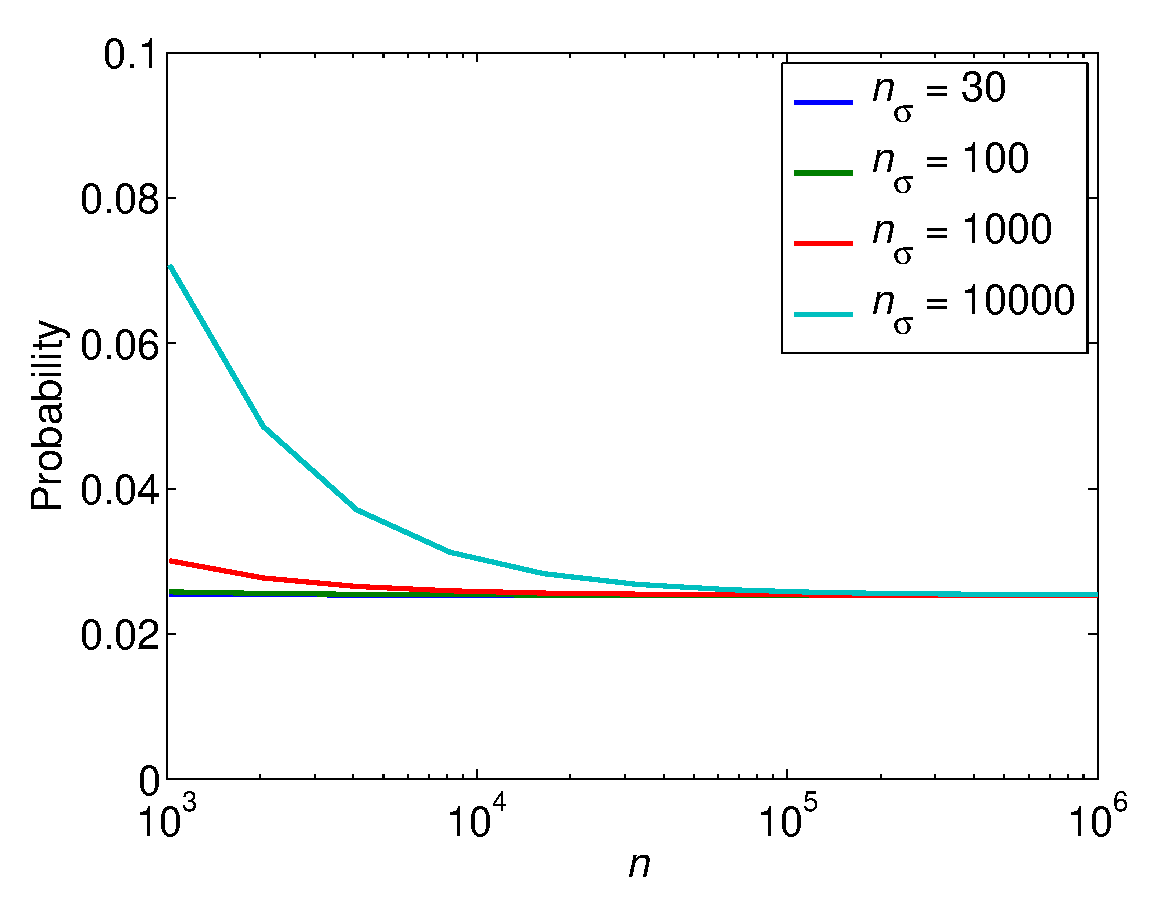
\includegraphics[width=3in]{probfailfig.eps}
\caption{The upper bound on the probability that $\hv_n \ge \hsigma^2$ in \eqref{probfail} for $\alpha_1 = 1 - \sqrt{95\%} \approx 2.5\%$ and $L=1.5$. \label{probfailfig}}
\end{figure}

\end{document}
